% begin module arcsin-properties
\begin{frame}
Important facts about $\Arcsin$:
\begin{columns}[c]
\column{.5\textwidth}
%\ 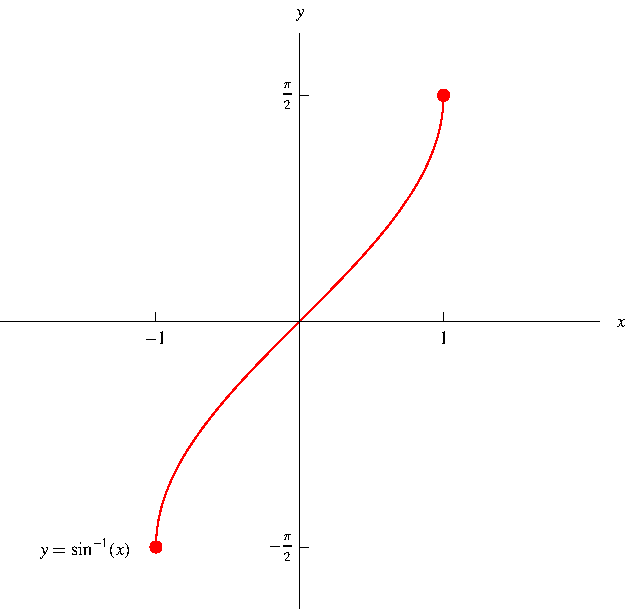
\includegraphics[height=6cm]{inverse-trig/pictures/07-06-arcsine.pdf}%
\psset{xunit=2cm,yunit=2cm}
\begin{pspicture}(-5,-1.4)(10,1.4)
\tiny
\psaxes[ticks=none, labels=none]{<->}(0,0)(-1.5,-2)(1.5,2)
\psLabels{1.5}{2}
\psLabelXOne
\psline(-1, -0.1)(-1,0.1)
\rput[t](-1,  -0.1){$-1$}

\psline(-0.1, 1.570796327)(0.1,1.570796327)
\rput[r](-0.1,  1.570796327){$\frac{\pi}{2}$}
\psline(-0.1, -1.570796327)(0.1,-1.570796327)
\rput[r](-0.1,  -1.570796327){$-\frac{\pi}{2}$}

\psplot[linecolor=red, plotpoints=1000]{-1}{1}{x ASIN}
\rput[rb](-0.05, 0.2){$y=\Arcsin x$} 
\psFullDot{1}{1.570796327}
\psFullDot{-1}{-1.570796327}
\uncover<3>{\psline[linecolor=red, linewidth=2pt]{<->}(-1,0)(1,0) }
\uncover<5>{\psline[linecolor=red, linewidth=2pt]{<->}(0,-1.570796327)(0,1.570796327) }

\end{pspicture}
\column{.5\textwidth}
\begin{enumerate}
\item  \alert<handout:0| 2-3>{Domain: \uncover<3->{$[-1, 1]$.}}
\item  \alert<handout:0| 4-5>{Range: \uncover<5->{$[-\pi /2, \pi /2]$.}}
\item  $\Arcsin x = y \Leftrightarrow \sin y = x$ and $-\pi /2 \leq y \leq \pi /2$.
\item  $\Arcsin (\sin x) = x$ for $-\pi /2 \leq x \leq \pi /2$.
\item  $\sin (\Arcsin x) = x$ for $-1 \leq x \leq 1$.
\item  $\frac{\diff}{\diff x} (\Arcsin x) = \frac{1}{\sqrt{1-x^2}}$.
\end{enumerate}
\end{columns}
\end{frame}
% end module arcsin-properties

